\documentclass[smaller]{beamer}
\usepackage{color}
\usepackage{ulem}

\usepackage{amsmath}
\usepackage{amssymb}
\usepackage{color}

\renewcommand{\familydefault}{\sfdefault}

% syntactic coloring
% by default, beamer-colors are
%    normal text is black on white.
%    alerted text is red.
%    example text is a dark green (green with 50% black).
%    structure is set to a light version of MidnightBlue (more precisely, 20% red, 20% green, and 70% blue).

\setbeamercolor{key point}{parent=alerted text}

\def\struct{\usebeamercolor[fg]{structure}}
\def\key{\em \usebeamercolor[fg]{key point}}
\def\aside{\scriptsize \usebeamercolor[fg]{example text}}
\def\newthing{\usebeamercolor[fg]{key point}}
\def\oldthing{\usebeamercolor[fg]{structure}}
\def\defthing{\usebeamercolor[fg]{structure}}

% \definecolor{blue}{rgb}{0.05,0.6,1}
% \definecolor{orange}{rgb}{1,0.549,0}
% \definecolor{dark-red}{rgb}{.4,.1,.1}
% \definecolor{pink}{rgb}{1,.8,.8}
% \definecolor{dark-green}{rgb}{.1,.6,.1}
% \definecolor{light-green}{rgb}{.8,1,.8}
% \definecolor{blue-white}{rgb}{.95,.95,1}
% \definecolor{purple}{rgb}{1, 0.0, 0.6}

\newcommand{\R}{\mathbb{R}}
\newcommand{\Q}{\mathbb{Q}}
\newcommand{\Z}{\mathbb{Z}}
\newcommand{\N}{\mathbb{N}}
\newcommand{\C}{\mathbb{C}}

\renewcommand{\P}{\mathbb{P}}
\newcommand{\E}{\mathbb{E}}

\newcommand{\var}{\mathop{\mbox{Var}}}
\newcommand{\cov}{\mathop{\mbox{cov}}}
\newcommand{\median}{\mathop{\mbox{median}}}
%\newcommand{\det}{\mathop{\mbox{det}}}
\newcommand{\supp}{\mathop{\mbox{supp}}}
\newcommand{\sgn}{\mathop{\mbox{sgn}}}

\newcommand{\conv}{\mathop{\mbox{conv}}}
\newcommand{\deq}{\stackrel{\scriptscriptstyle{d}}{=}}
\newcommand{\dcv}{\stackrel{\scriptscriptstyle{d}}{\longrightarrow}}


\newcommand{\figcredit}[1]{{\begin{flushright}\usebeamercolor[fg]{structure} \it \tiny #1 \end{flushright}}}



\def\basedir{files}

\newcommand{\widebar}[1]{\overline{#1}}
\newcommand{\finger}{ \vtop{ \vskip-5pt \hbox{ 
\includegraphics[width=.68in]{finger_right}} } }

\renewcommand<>{\sout}[1]{
  \only#2{\beameroriginal{\sout}{#1}}
  \invisible#2{#1}
}
\setbeamertemplate{blocks}[default]
\usecolortheme{rose}

\mode<presentation>
{
  % \usetheme{default}
  \usetheme{boxes}
  % or ...
  \usefonttheme[options]{structuresmallcapsserif}

  \setbeamercovered{transparent}
  % or whatever (possibly just delete it)
}


\usepackage[english]{babel}
% or whatever

%% PLR COMMENTED THESE:
\usepackage[latin1]{inputenc}
% \usepackage{times}
% \usepackage[T1]{fontenc}
% Or whatever. Note that the encoding and the font should match. If T1
% does not look nice, try deleting the line with the fontenc.


\title % (optional, use only with long paper titles)
{ Using local PCA to summarize how relatedness varies along the genome }


\author % (optional, use only with lots of authors)
{Peter Ralph and Han Li}

\institute[UO]
{
    University of Oregon -- Institute of Ecology and Evolution \\
    \textit{and} University of Southern California
  }

\date % (optional)
{June 26, 2017\\
\vspace{1em}
bioRxiv:070615}


\begin{document}


\begin{frame}
  \titlepage
\end{frame}



%%%%%%%%
\begin{frame}{Principal Components Analysis (PCA)}

    \includegraphics<1>[width=0.9\textwidth]{\basedir/novembre-map-genes-mirror-geography-crop}

    \only<1>{\aside (Novembre et al 2008)}

    \includegraphics<2>[width=\textwidth]{\basedir/maize_pca}

    \only<2>{\aside (van Heerwaarden et al 2010)}
    % http://www.pnas.org/content/108/3/1088.full

\end{frame}

%%%%%%%%
\begin{frame}{\ldots describes the covariance matix}

    Genetic covariance between samples $i$ and $j$ is \\
    the {average} over {\newthing loci} \\
    and {\newthing reference samples} $x$, $y$ of:

    \begin{center}
        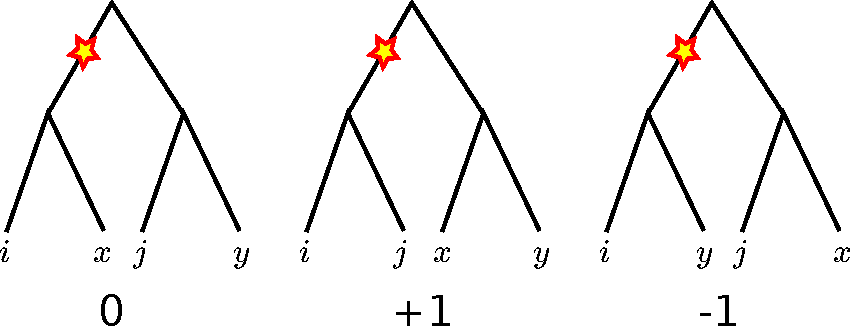
\includegraphics[width=\textwidth]{\basedir/what_is_covariance}
    \end{center}

    \ldots so summarizes average {\newthing patterns of relationships} \\
    caused by {\oldthing population structure}.

\end{frame}

%%%%%%%%
\begin{frame}{``Population structure''}
    \vspace{1em}
    is historical patterns of interbreeding, migration, and population sizes.

    \vspace{2em}
    \pause

    but: {\Large linked selection} \\
    \vspace{1em}
    {\newthing locally distorts} resulting genealogical patterns. \\
    ex: local adaptation, or background selection.

    \vspace{2em}
    \pause

  \begin{overlayarea}{\textwidth}{0.4\textheight}
    \only<3>{
    \begin{center}
        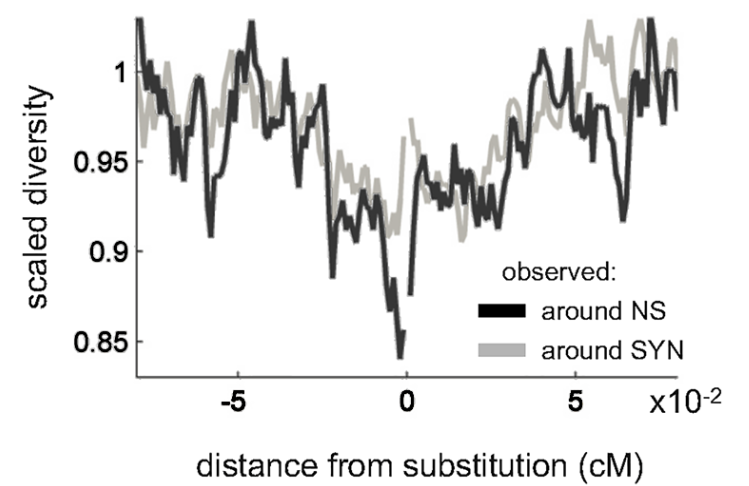
\includegraphics[width=0.5\textwidth]{\basedir/elyashiv-2016-drosophila-linked-sel}
    \end{center}
    {\aside (Elyashiv et al 2016)}
    }
      \only<4>{
          \begin{center}
              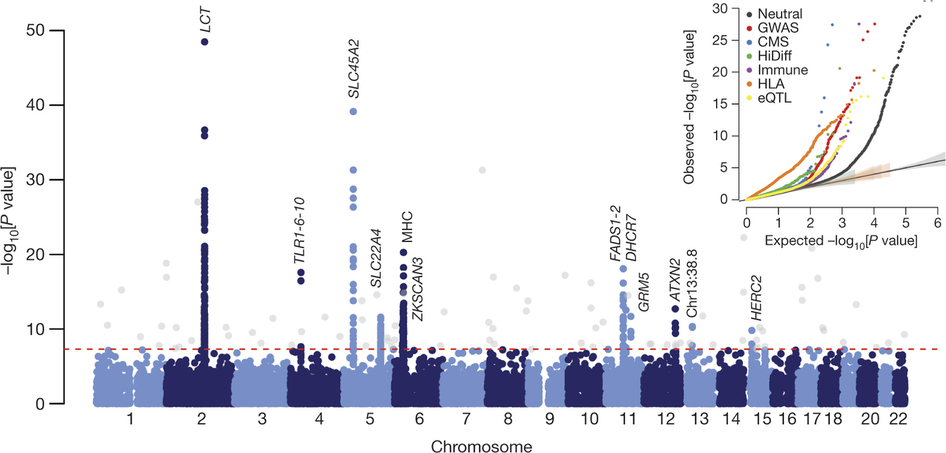
\includegraphics[width=0.8\textwidth]{\basedir/mathieson-genome-scan}
          \end{center}
          {\aside (Mathieson et al 2015)}
      }
      \only<5>{
          \vspace{4em}
          {\Large Goal:} describe shared, {\newthing large-scale} variation variation.
      }
  \end{overlayarea}

\end{frame}

% %%%%%%%%
% \begin{frame}{``Population structure''}
% 
%     \ldots  describes how everyone is related?
% 
%     \vspace{2em}
% 
%     \begin{itemize}
% 
%         \item  \alert{But:} local adaptation or hybridization
% 
%             \begin{itemize}
%                 \item leads to selection against migrants
%                 \item and differential gene flow.
%             \end{itemize}
% 
%         \item \alert{But:} background selection 
%             \begin{itemize}
%                 \item  makes coalescence faster near constrained sites.
%             \end{itemize}
% 
%     \end{itemize}
% 
%     \vspace{2em}
% 
%     \ldots so what is population structure?
% 
% \end{frame}


%%%%%%%%
\begin{frame}{Our method}

    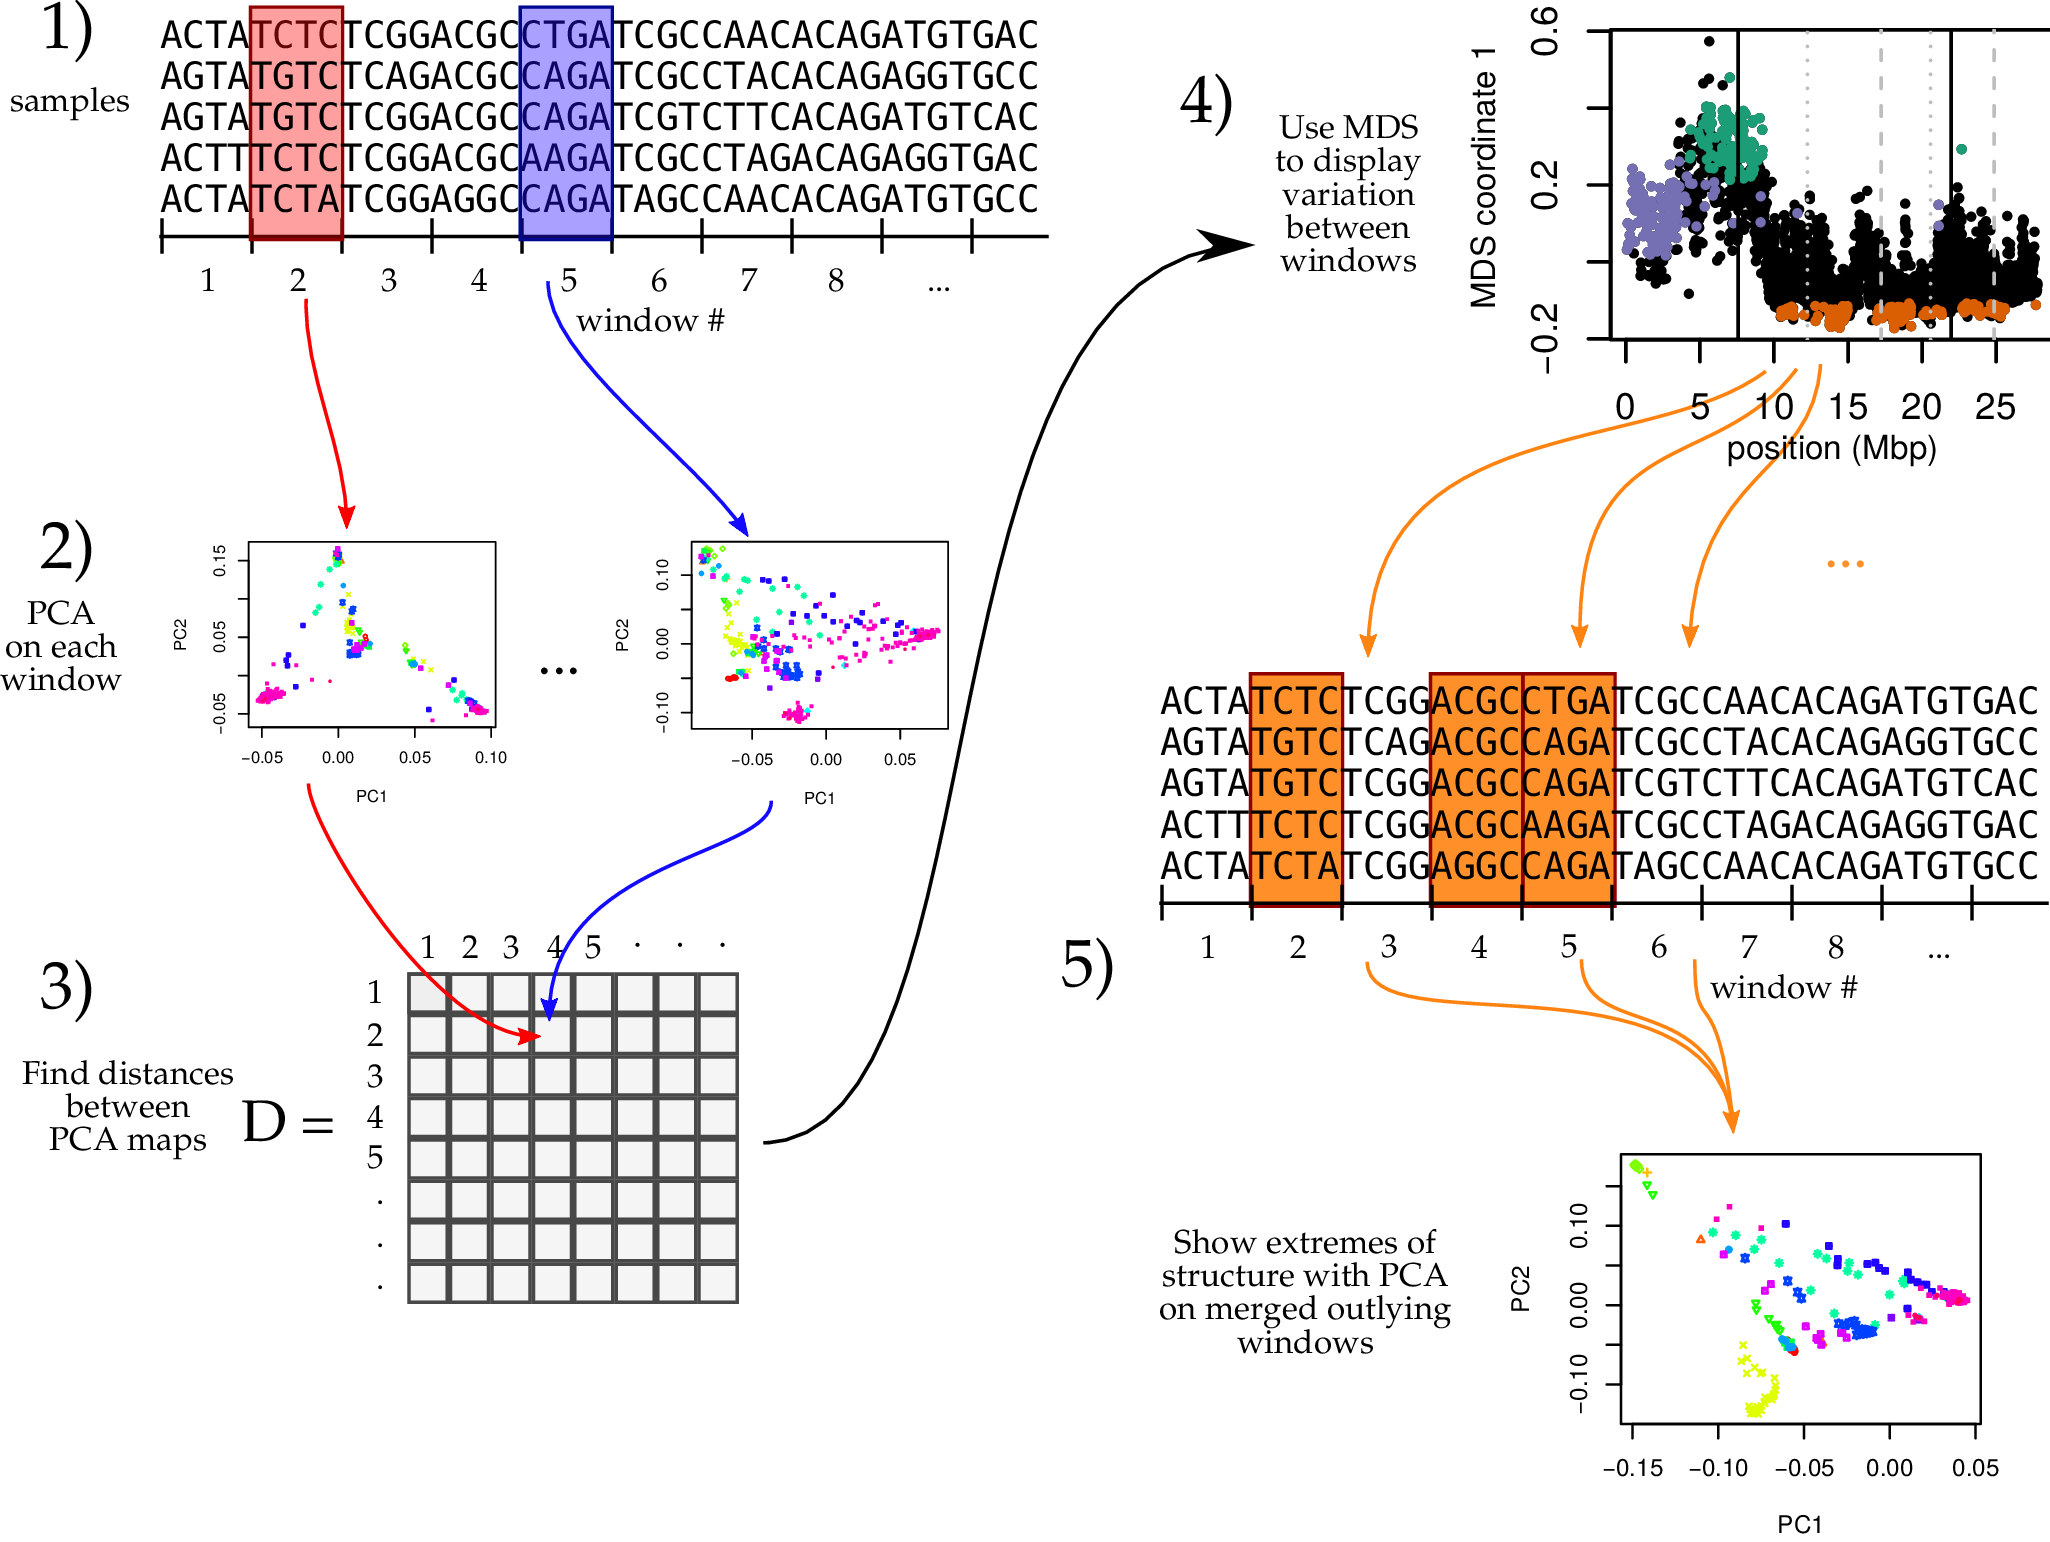
\includegraphics[width=\textwidth]{\basedir/the-method-diagram-modified}

\end{frame}


%%%%%%%%
\begin{frame}{``lostruct''}

    \begin{columns}
        \begin{column}{0.5\textwidth}
    \begin{itemize}
        \item an R package
        \item with templated Rmarkdown reports
        \item and a script interface
        \item \url{https://github.com/petrelharp/local_pca}
    \end{itemize}
        \end{column}
        \begin{column}{0.5\textwidth}
    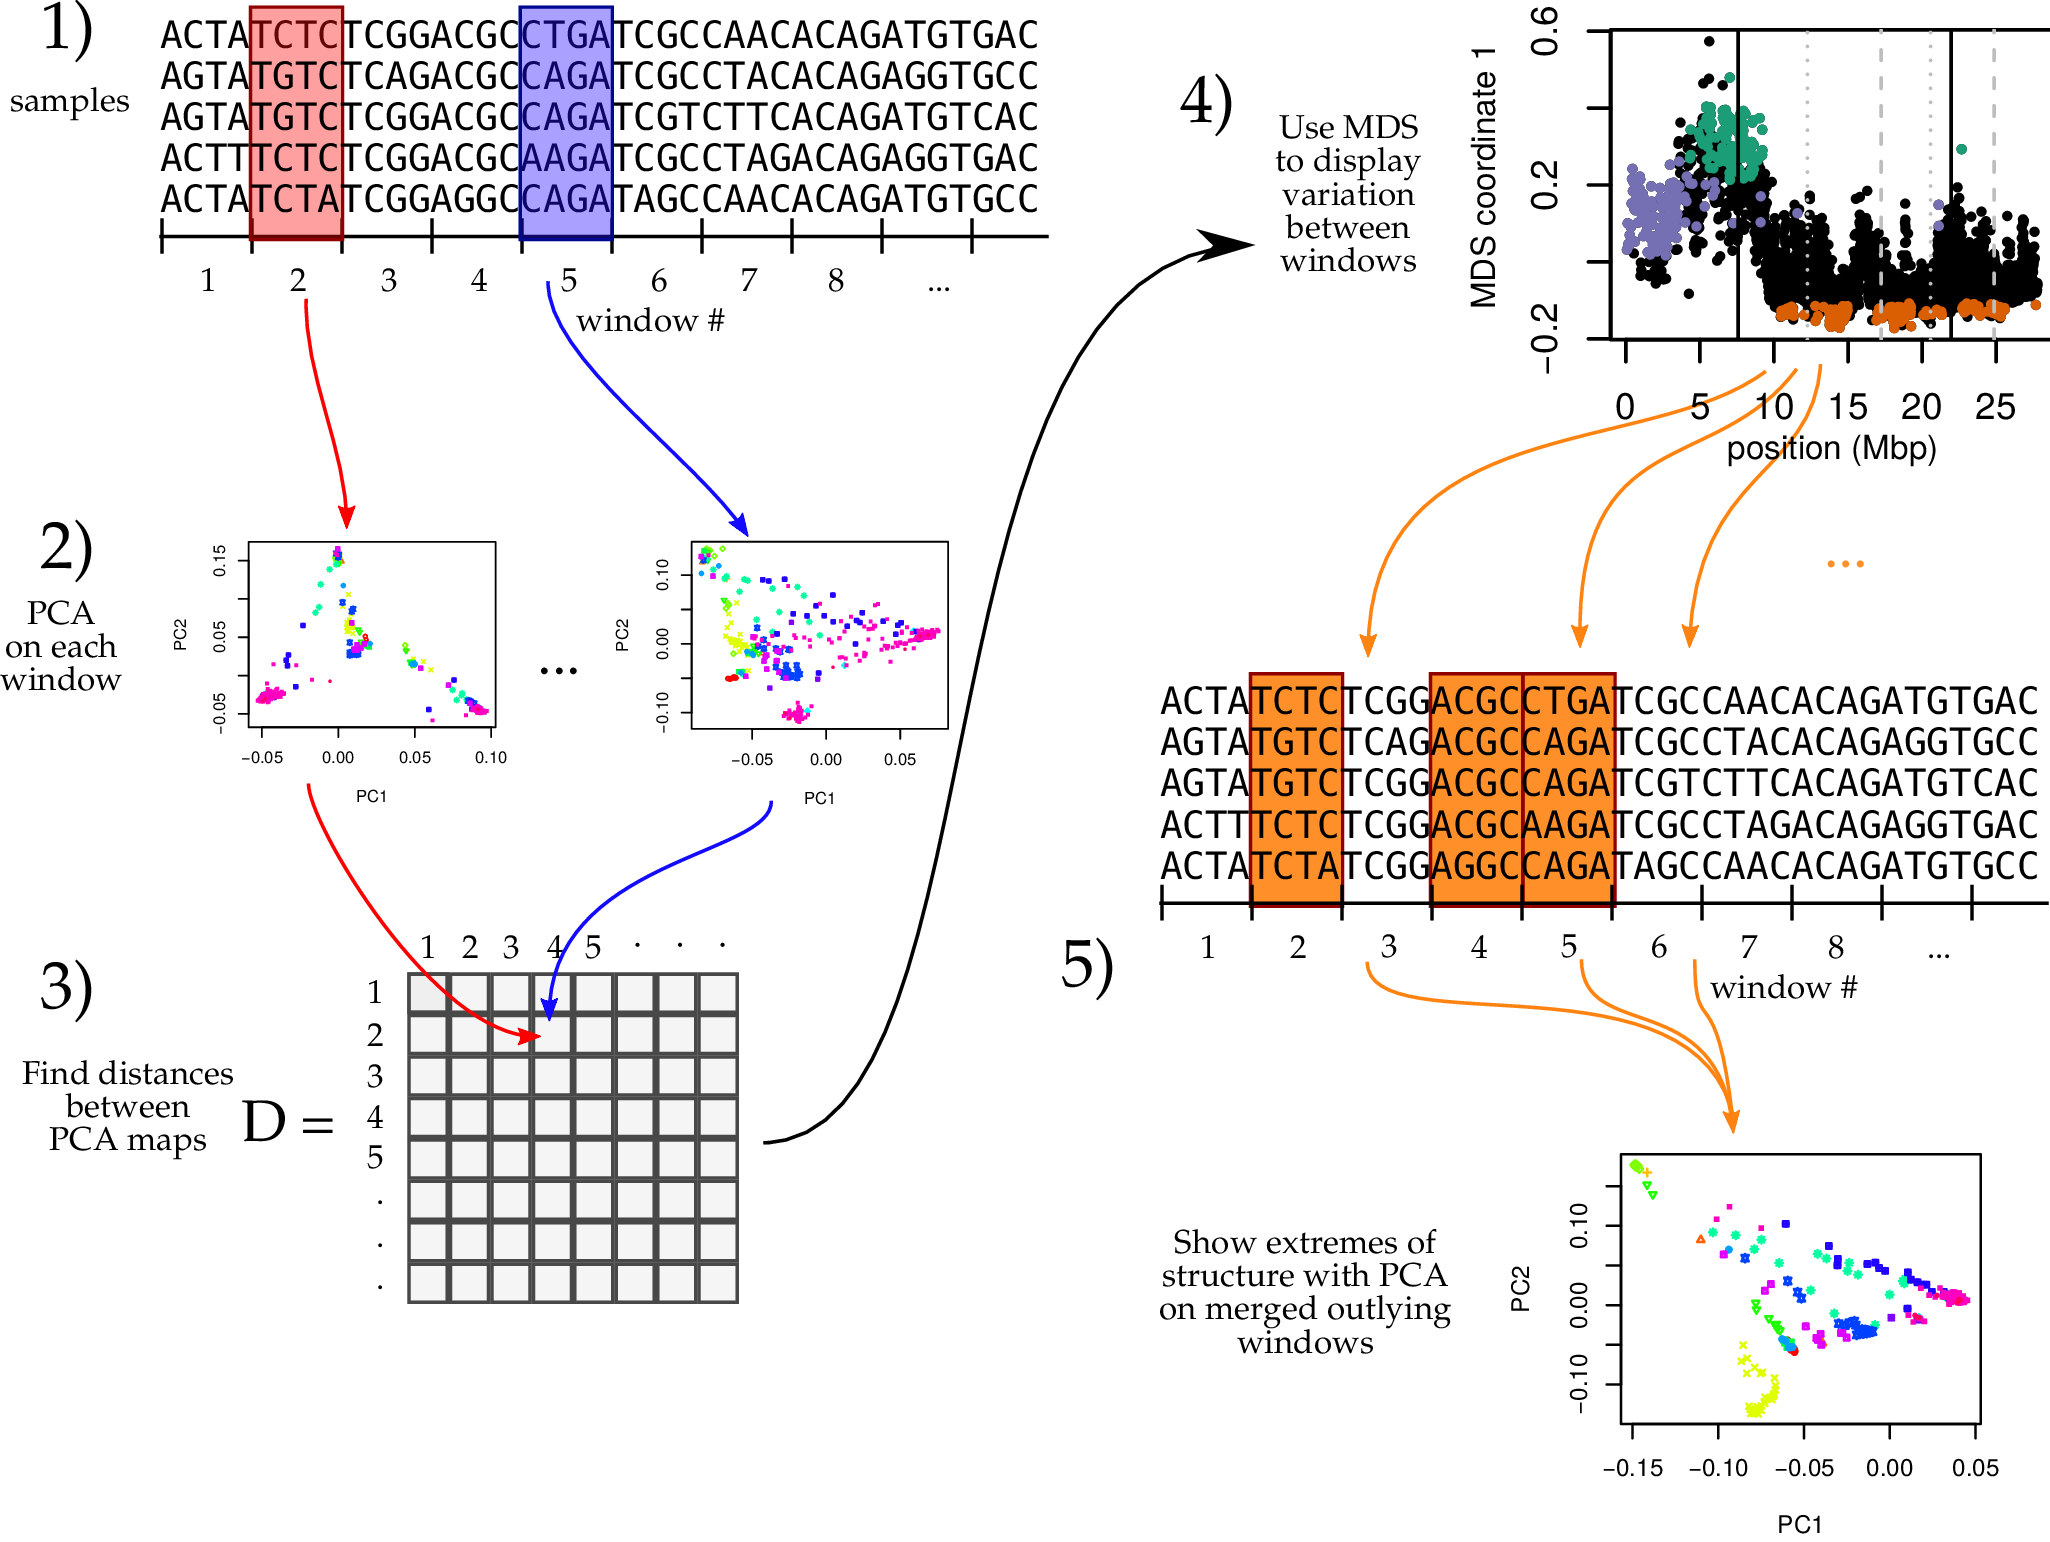
\includegraphics[width=\textwidth]{\basedir/the-method-diagram-modified}
        \end{column}
    \end{columns}

\end{frame}

%%%%%%%%
\begin{frame}{Simulation: local adaptation}

    \begin{itemize}
    \item three populations: (hot, dry) -- (hot, wet) -- (cold, wet) 

    \item clustered genes: (hot/cold) -- (wet/dry)

    \item 1000 diploids in each population and 1\% migration
    \item 25MB (0.625M) with 1000 evenly spaced loci with $s=\pm0.001$, 
    \item with simuPOP + msprime

    \end{itemize}

     % cp /home/peter/projects/pca/local_pca/sims/./local/threeway_sym_1000_1000_0.001_10.0_2.5e-8_4_21110/bp_2000_npc_2/figure/run-summary/plot_corners-1.pdf  ../writeup/talk/files/threeway_sym_1000_1000_0.001_10.0_2.5e-8_4_21110_bp_2000_npc_2_plot_corners-1.pdf
     % ln -s threeway_sym_1000_1000_0.001_10.0_2.5e-8_4_21110_bp_2000_npc_2_plot_corners-1.pdf files/sym_threeway_corners.pdf
     \includegraphics<1>[width=\textwidth]{\basedir/sym_threeway_corners}
     % cp /home/peter/projects/pca/local_pca/sims/./local/threeway_sym_1000_1000_0.001_10.0_2.5e-8_4_21110/bp_2000_npc_2/figure/run-summary/plot_corner_pca-1_1_2.pdf  ../writeup/talk/files/threeway_sym_1000_1000_0.001_10.0_2.5e-8_4_21110_bp_2000_npc_2_plot_corner_pca-1_1_2.pdf
     % ln -s threeway_sym_1000_1000_0.001_10.0_2.5e-8_4_21110_bp_2000_npc_2_plot_corner_pca-1_1_2.pdf files/sym_threeway_pca.pdf
     \includegraphics<2>[width=\textwidth]{\basedir/sym_threeway_pca}


\end{frame}

%%%%%%%%
\begin{frame}{Data: African \textit{D.~melanogaster} }

    \begin{itemize}
        \item DPGP {\aside (Langley et al 2012; Pool et al 2012; Lack et al 2015)} \\
        \item 380 mostly African samples -- WGS -- 9 Kb windows
        \item<2-> large, segregating inversions {\aside (Corbett-Detig \& Hartl 2012; Langley et al 2012)}
        \item<3-> without less common inversion haplotypes: {\newthing linked selection?}
    \end{itemize}

    \vspace{2em}

  \begin{overlayarea}{\textwidth}{0.55\textheight}

    \begin{center}
        \includegraphics<2>{\basedir/drosophila_just_2R_3L}
        \includegraphics<3>[width=\textwidth]{\basedir/drosophila_recomb_mds_for_talk}
    \end{center}

      \end{overlayarea}

\end{frame}

% %%%%%%%%
% \begin{frame}{Data: European Humans}
% \end{frame}


%%%%%%%%
\begin{frame}{Data: \textit{Medicago truncatula} Hapmap {\aside (Tang et al 2014)}}

    \begin{itemize}
        \item 263 pan-Mediterranean samples -- WGS -- 100 Kb windows
    \end{itemize}

  \begin{overlayarea}{\textwidth}{0.9\textheight}
      \begin{center}
      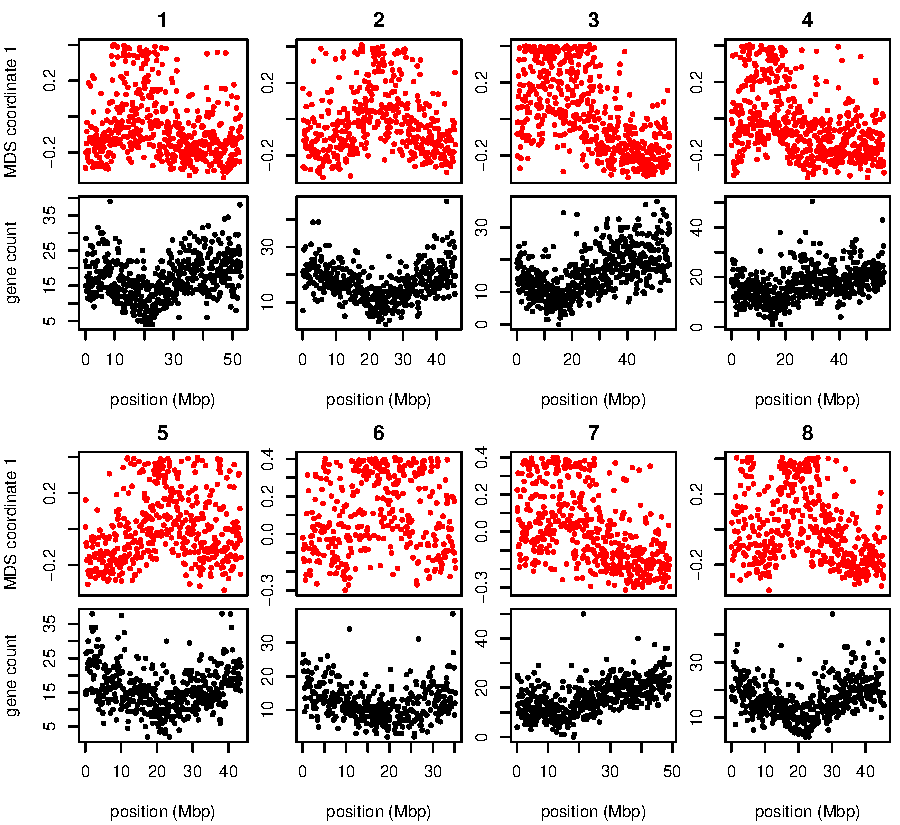
\includegraphics[height=0.8\textheight]{\basedir/medicago_for_talk}
      \end{center}
  \end{overlayarea}

\end{frame}


%%%%%%%%
\begin{frame}{Conclusions}

    \begin{columns}
        \begin{column}{0.7\textwidth}
    \begin{itemize}
        \item  there isn't always a single ``population structure''

        \item (more) evidence for widespread effects of linked selection

        \item \texttt{lostruct} is a visualization tool

        \item applicable to other summary strategies

        \item try it out: \url{https://github.com/petrelharp/local_pca}
    \end{itemize}
        \end{column}
        \begin{column}{0.4\textwidth}
    
            \vspace{-3em}
    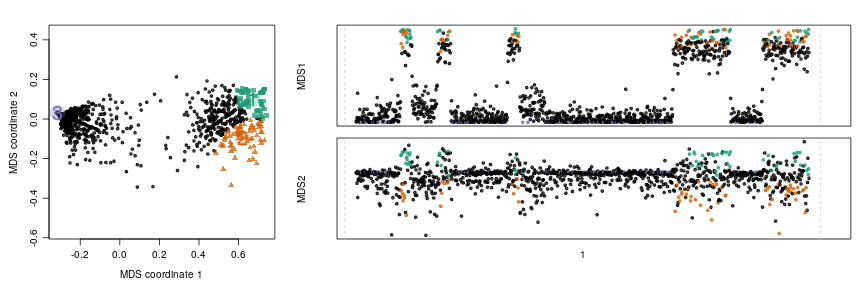
\includegraphics[angle=270,width=0.75\textwidth]{\basedir/another_example_sim}
        \end{column}
    \end{columns}
\end{frame}

%%%%%%%%
\begin{frame}{Thanks}
    \begin{columns}
        \begin{column}{0.6\textwidth}

    {\Large Han Li} -- USC  --  bioRxiv:070615

            \begin{center}
            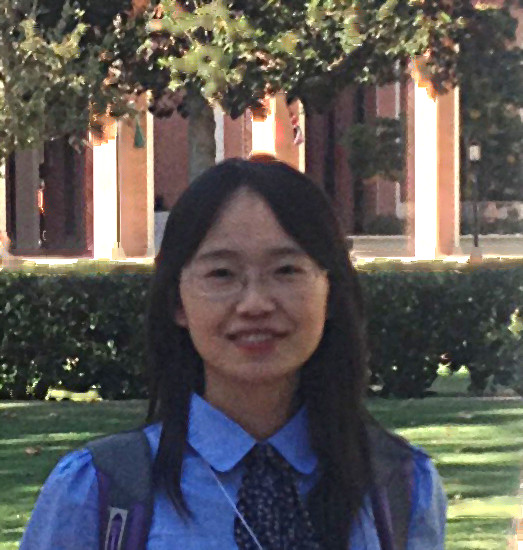
\includegraphics[width=0.6\textwidth]{\basedir/hanli}
            \end{center}


    John Pool, Russ Corbett-Detig \\
    Peter Chang, Matilde Cordeiro \\
    Graham Coop, Jeremy Berg, Yaniv Brandvain, Chuck Langley  \\
    Jaime Ashander, Jerome Kelleher

    \vspace{1em}

    \textbf{Funding:} \\
    NSF ABI 

        \end{column}
        \begin{column}{0.4\textwidth}

            \only<2->{

                \begin{center}
            \textbf{University of Oregon} \\
    
            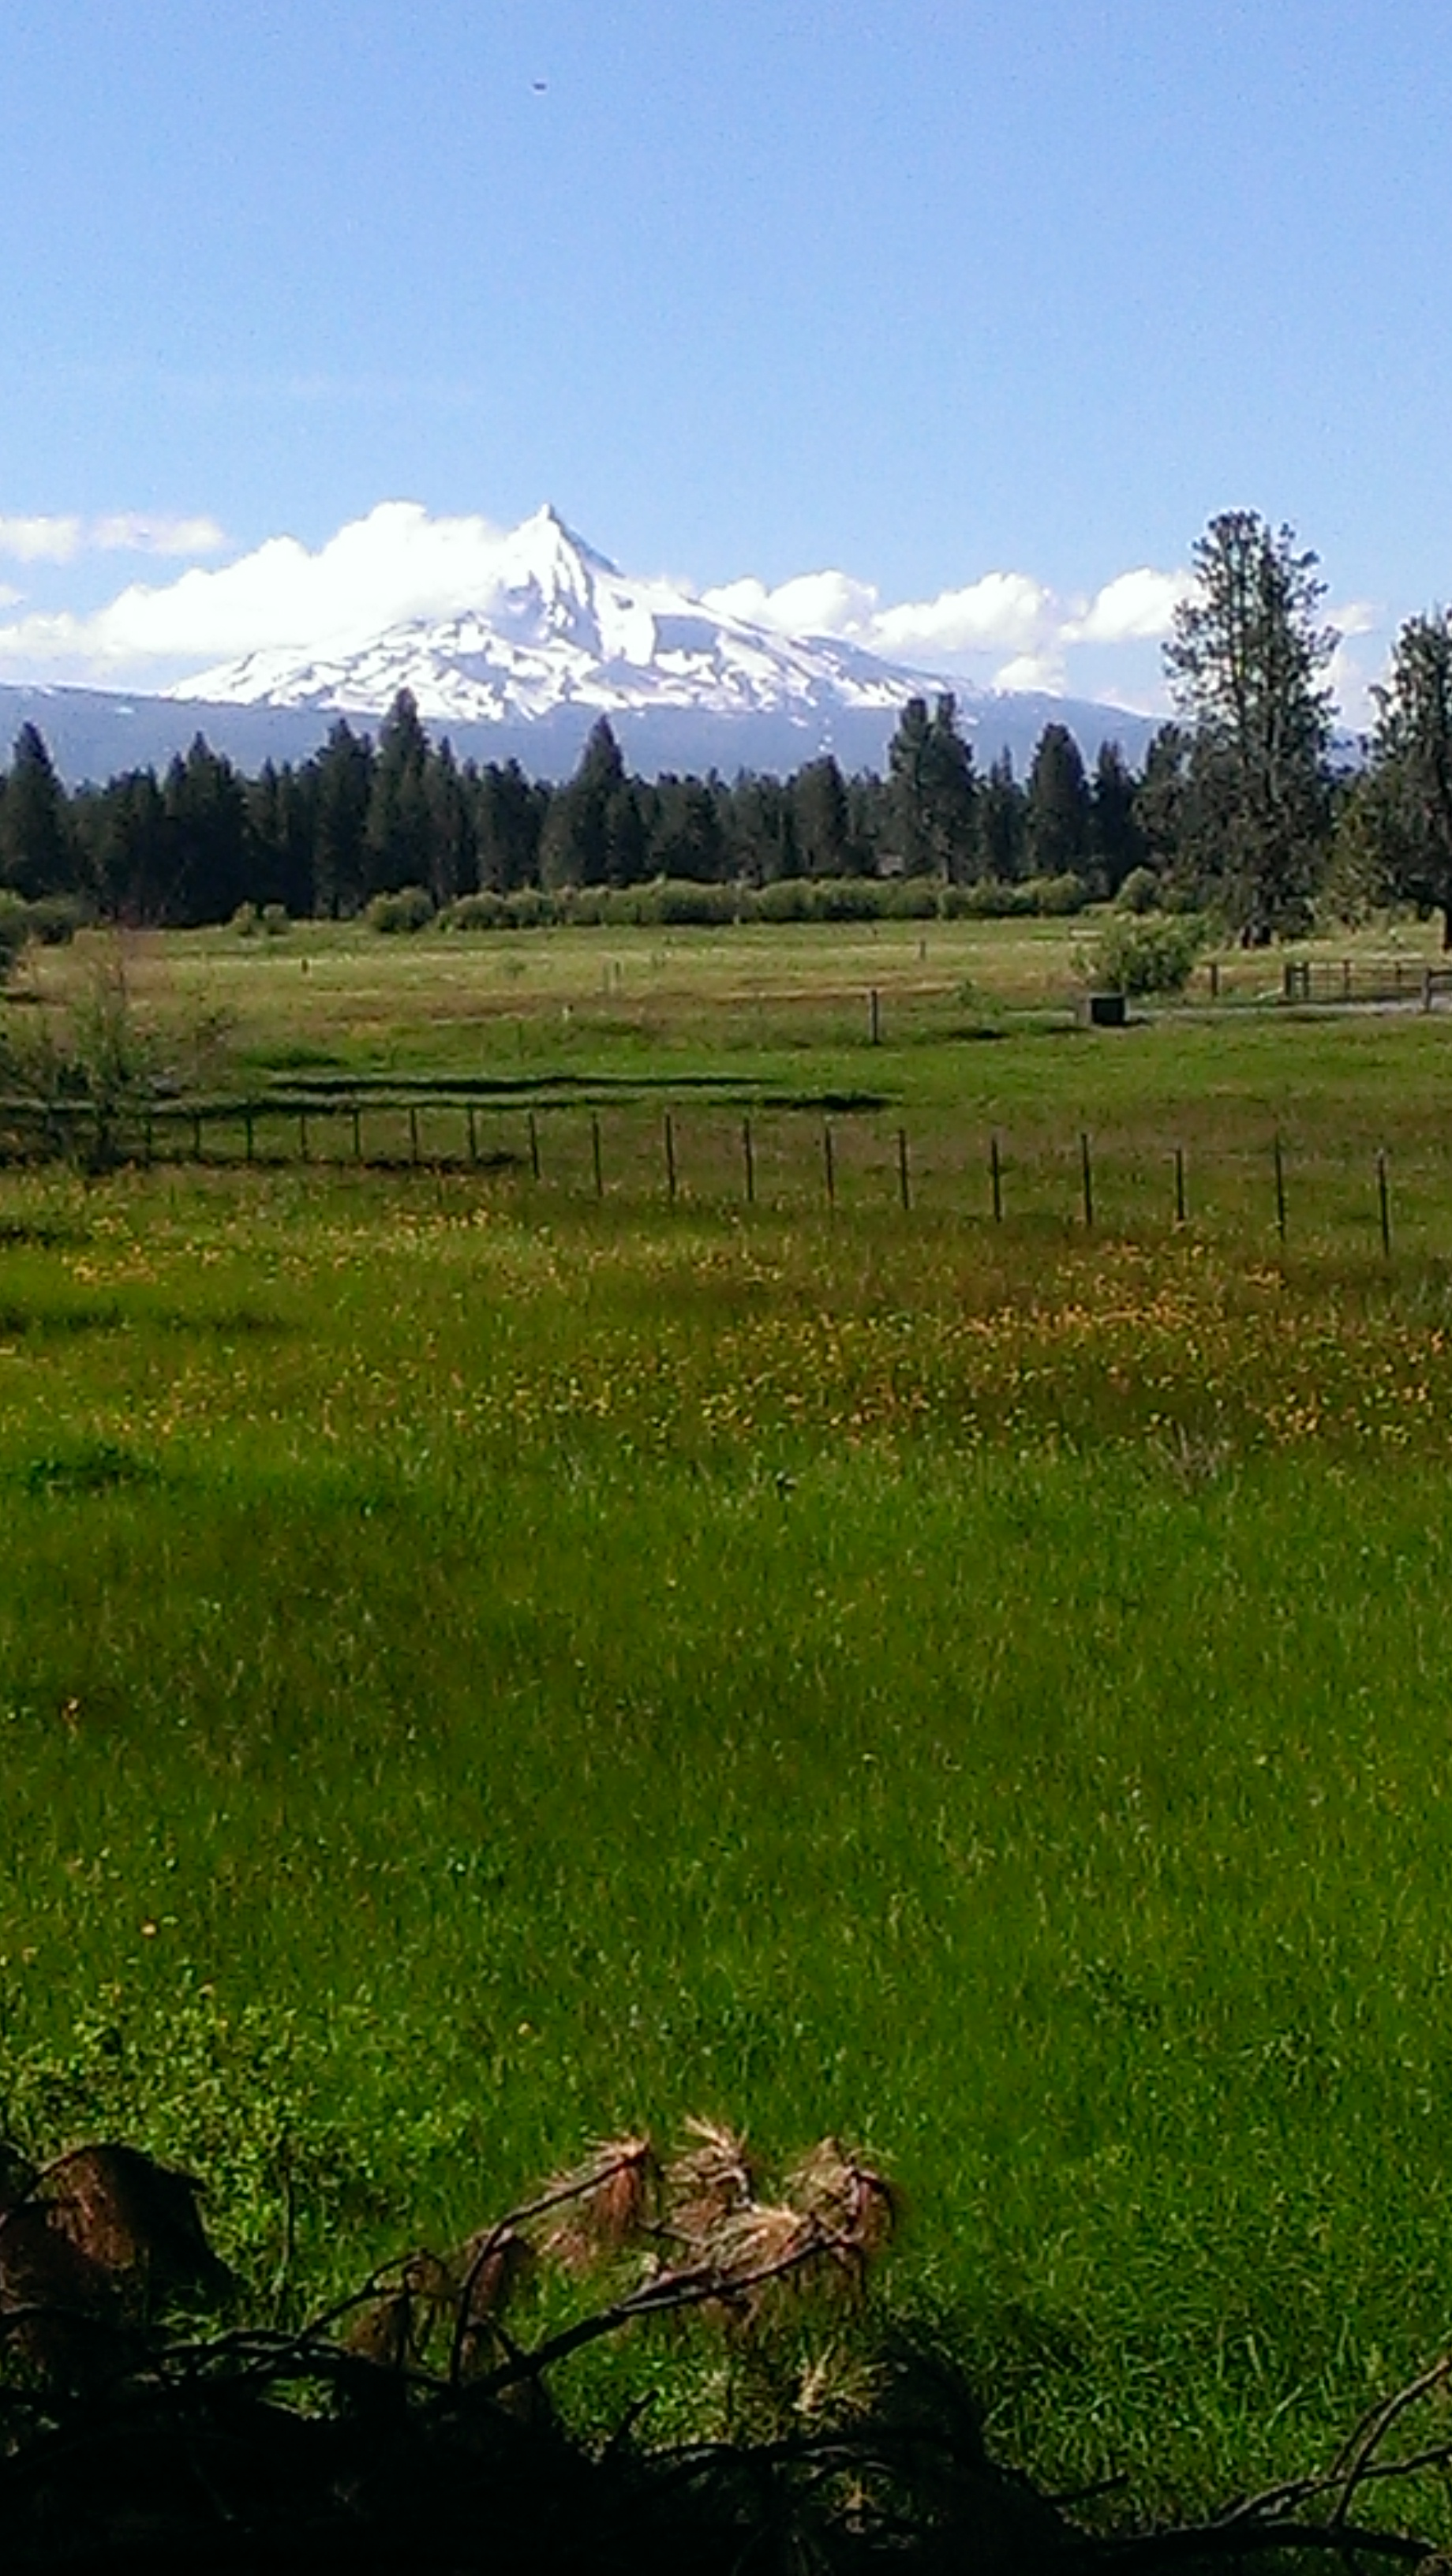
\includegraphics[width=\textwidth]{\basedir/oregon}
                \end{center}
        }
        \end{column}
    \end{columns}

\end{frame}


%%%%%%%%
\begin{frame}{Robust?}

    \begin{itemize}

        \item PC switching? \\
            uses distance metric insensitive to PC order

        \item window choice? \\
            weakly: method selects size maximizing information while minimizing noise

        \item mutation rate variation? 
            \\ normalizes by matrix norm to capture just structure

        \item recombination rate variation?
            \\ do windows in cM if possible
            \\ else inversions $\approx$ low recomb regions

        \item missing data?
            \\ filter; but user beware
    \end{itemize}

\end{frame}

\end{document}
